\documentclass[a4paper]{article}
    \usepackage[pdftex]{hyperref}
    \usepackage[latin1]{inputenc}
    \usepackage[english]{babel}
    \usepackage{a4wide}
    \usepackage{amsmath}
    \usepackage{amssymb}
    \usepackage{algorithmic}
    \usepackage{algorithm}
    \usepackage{ifthen}
    \usepackage{listings}
    % move the asterisk at the right position
    \lstset{basicstyle=\ttfamily,tabsize=4,literate={}{${}^{}$}1}
    %\lstset{language=C,basicstyle=\ttfamily}
    \usepackage{moreverb}
    \usepackage{palatino}
    \usepackage{multicol}
    \usepackage{tabularx}
    \usepackage{comment}
    \usepackage{verbatim}
    \usepackage{color}
    
    % Because of an error on line 41 I added this
    \usepackage{graphicx}
    
    % Used for drawing DFAs and NFAs
    \usepackage{tikz}
    \usetikzlibrary{automata, positioning}
    
    %% pdflatex?
    \newif\ifpdf
    \ifx\pdfoutput\undefined
    \pdffalse % we are not running PDFLaTeX
    \else
    \pdfoutput=1 % we are running PDFLaTeX
    \pdftrue
    \fi
    %\ifpdf
    %\usepackage[pdftex]{graphicx}
    %\else
    %\usepackage{graphicx}
    %\fi
    \ifpdf
    \DeclareGraphicsExtensions{.pdf, .jpg}
    \else
    \DeclareGraphicsExtensions{.eps, .jpg}
    \fi
    
    \parindent=0cm
    \parskip=0cm
    
    \setlength{\columnseprule}{0.4pt}
    \addtolength{\columnsep}{2pt}
    
    \addtolength{\textheight}{5.5cm}
    \addtolength{\topmargin}{-26mm}
    \pagestyle{empty}
    
    %%
    %% Sheet setup
    %% 
    \newcommand{\coursename}{Formal Languages and Logic}
    \newcommand{\courseno}{CO21-320211}
     
    \newcommand{\sheettitle}{Homework}
    \newcommand{\mytitle}{}
    \newcommand{\mytoday}{\textcolor{blue}{September 16th}, 2018}
    
    % Current Assignment number
    \newcounter{assignmentno}
    \setcounter{assignmentno}{2}
    
    % Current Problem number, should always start at 1
    \newcounter{problemno}
    \setcounter{problemno}{1}
    
    %%
    %% problem and bonus environment
    %%
    \newcounter{probcalc}
    \newcommand{\exercise}[2]{
      \pagebreak[2]
      \setcounter{probcalc}{#2}
      ~\\
      {\large \textbf{Exercise \textcolor{blue}{\arabic{problemno}}} \hspace{0.2cm}\textit{#1}} \refstepcounter{problemno}\vspace{2pt}\\}
    
    \newcommand{\bonus}[2]{
      \pagebreak[2]
      \setcounter{probcalc}{#2}
      ~\\
      {\large \textbf{Bonus Problem \textcolor{blue}{\arabic{assignmentno}}.\textcolor{blue}{\arabic{problemno}}} \hspace{0.2cm}\textit{#1}} \refstepcounter{problemno}\vspace{2pt}\\}
    
    %% some counters  
    \newcommand{\assignment}{\arabic{assignmentno}}
    
    %% solution  
    \newcommand{\solution}{\pagebreak[2]{\bf Solution:}\\}
    
    %% Hyperref Setup
    \hypersetup{pdftitle={Homework \assignment},
      pdfsubject={\coursename},
      pdfauthor={},
      pdfcreator={},
      pdfkeywords={Formal Languages and Logic},
      %  pdfpagemode={FullScreen},
      %colorlinks=true,
      %bookmarks=true,
      %hyperindex=true,
      bookmarksopen=false,
      bookmarksnumbered=true,
      breaklinks=true,
      %urlcolor=darkblue
      urlbordercolor={0 0 0.7}
    }
    
    \begin{document}
    \coursename \hfill Course: \courseno\\
    Jacobs University Bremen \hfill \mytoday\\
    \textcolor{blue}{Dragi Kamov and Dushan Terzikj}\hfill
    \vspace*{0.3cm}\\
    \begin{center}
    {\Large \sheettitle{} \textcolor{blue}{\assignment}\\}
    \end{center}
    
    \exercise{}{0}
    \solution
    \textcolor{blue}{
        Let us define a DFA, $A=(Q, \Sigma, \delta, q_0, F)$, where:
        \begin{itemize}
            \item $Q=\{q_i|i\in\mathbb{N}$ and $\forall{i}\in\ [0,4]\}$
            \item $\Sigma=\{a, b\}$
            \item $\delta :\Sigma\times Q\rightarrow Q$,\\$\delta=\{((q_0, a), q_1),((q_0, b), q_2),((q_1, a), q_1),((q_1, b), q_3),((q_2, a), q_4),((q_2, b), q_2),((q_3, a), q_1),((q_4, b), q_2),\\((q_3, b), q_3),((q_4, a), q_4)\}$
            \item Starting state is $q_0$
            \item $F=\{q_1, q_2\}$
        \end{itemize}
        \textbf{Transition table}\\ \\
        \begin{tabular}{|c|c|c|}
            \hline
            &\textbf{a}&\textbf{b}  \\
            \hline
            \textbf{$q_0$}&$q_1$&$q_2$  \\
            \hline
            \textbf{$q_1$}&$q_1$&$q_3$  \\
            \hline
            \textbf{$q_2$}&$q_4$&$q_2$  \\
            \hline
            \textbf{$q_3$}&$q_1$&$q_3$  \\
            \hline
            \textbf{$q_4$}&$q_4$&$q_2$  \\
            \hline
        \end{tabular}\\ \\
        \textbf{Graph}\\ \\
        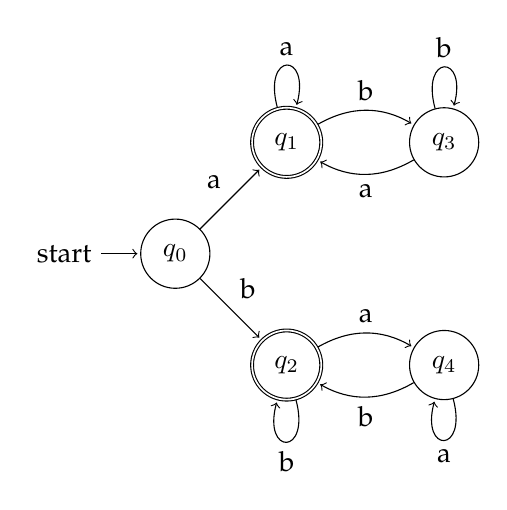
\begin{tikzpicture}[shorten >=1pt, node distance=2cm, on grid, auto]
           \node[state, initial](q_0){$q_0$};
           \node[state, accepting](q_1)[above right=of q_0]{$q_1$};
           \node[state, accepting](q_2)[below right=of q_0]{$q_2$};
           \node[state](q_3)[right=of q_1]{$q_3$};
           \node[state](q_4)[right=of q_2]{$q_4$};
           \path[->]
           (q_0)    edge node {a} (q_1)
                    edge node {b} (q_2)
            (q_1)   edge [loop above] node {a} ()
                    edge [bend left=30] node {b} (q_3)
            (q_2)   edge [loop below] node {b} ()
                    edge [bend left=30] node {a} (q_4)
            (q_3)   edge [bend left=30] node {a} (q_1)
                    edge [loop above] node {b} ()
            (q_4)   edge [bend left=30] node {b} (q_2)
                    edge [loop below] node {a} ();
        \end{tikzpicture}
    }
    
    \exercise{}{0}
    \solution
    \textcolor{blue}{
    We have three states and they are all accepting states. With 1 we are always going to the next state, but with 0 we could either stay in the same state or go to the next state. When we would reach the third state, the 0 would always give us the same current state and the 1 is not defined.}
    
    \newpage
    \exercise{}{0}
    \solution
    \textcolor{blue}{
    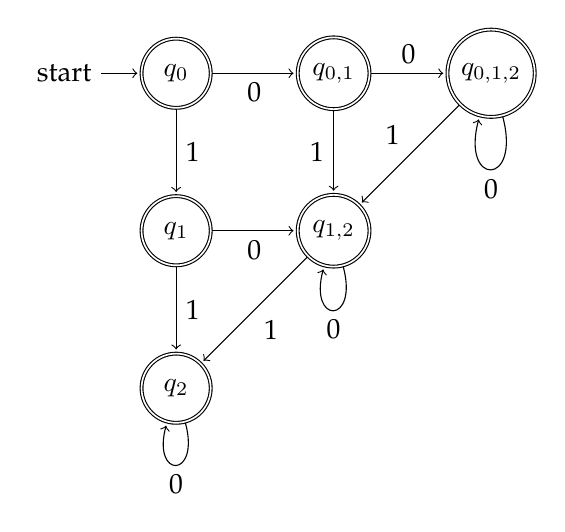
\begin{tikzpicture}[shorten >=1pt,node distance=2cm,on grid,auto] 
       \node[state,initial,accepting] (q_0)   {$q_0$}; 
       \node[state,accepting] (q_1) [below=of q_0] {$q_1$}; 
       \node[state,accepting] (q_2) [below=of q_1] {$q_2$}; 
       \node[state,accepting](q_{0,1}) [right=of q_0] {$q_{0,1}$};
       \node[state,accepting](q_{1,2}) [right=of q_1] {$q_{1,2}$};
       \node[state,accepting](q_{0,1,2}) [right=of q_{0,1}] {$q_{0,1,2}$};
        \path[->] 
        (q_0) edge  node {1} (q_1)
              edge  node [swap] {0} (q_{0,1})
        (q_1) edge  node  {1} (q_2)
              edge  node [swap] {0} (q_{1,2})
        (q_2) edge [loop below] node {0} ()
        (q_{0,1}) edge node {0} (q_{0,1,2})
            edge node [swap] {1} (q_{1,2})
        (q_{1,2}) edge node {1} (q_2)
            edge [loop below] node {0} ()
        (q_{0,1,2}) edge [loop below] node {0} ()
            edge node [swap] {1} (q_{1,2});
    \end{tikzpicture}}
    
    \end{document}